\documentclass[11pt,a4paper,toc=bibliography,toc=listof,titlepage=firstiscover]{scrreprt}
\usepackage[utf8]{inputenc}
\usepackage{array}
\usepackage{blindtext}
\usepackage{graphicx}
\usepackage{subcaption}
\usepackage[T1]{fontenc}
\usepackage{setspace}
\usepackage{pdfsync}
\usepackage{blindtext}
\usepackage[ngerman]{babel}
\usepackage{booktabs}
\usepackage{xcolor}
\usepackage{multirow}
%Schriftarten hier definieren
\usepackage{lmodern}
%\usepackage{tgheros}
%\renewcommand*\familydefault{\sfdefault}
%\usepackage{tgpagella}
\usepackage[babel,german=guillemets]{csquotes}
\usepackage[style=apa]{biblatex}
\usepackage{hyperref}
\usepackage{csquotes}
\addbibresource{resources/literatur.bib}
\hypersetup{colorlinks=true, linkcolor=black, urlcolor=black, citecolor=black}
%Abstand der Einträge im Literaturverzeichnis als em
\setlength\bibitemsep{0.75em}
%Kein Einzug bei einem neuen Absatz
\setlength{\parindent}{0mm}
%Inhaltsverzeichnis ohne eigene Seitenzahl
\AtBeginDocument{\addtocontents{toc}{\protect\thispagestyle{empty}}} 
\usepackage[left=3cm,right=2.5cm,top=2.5cm,bottom=2cm]{geometry}

%Daten des Deckblatts
  \titlehead
  {
    {
      \begin{center}
        \vspace{2.5cm}
        
\includegraphics[scale=0.3]{resources/nak-logo.png}
      \end{center}
    }
  	%M.Sc. Angewandte Informatik
  }
  \subject{Hausarbeit}
  \title{Integration der Data Science in Organisationen / Abteilungen}
    \subtitle{Vorlesung Data-Science Projektorganisation}
    \author{Leon Henne}
  \date{\small{Köln, den \today}}
  \publishers{Betreut durch Prof. Dr. Michael Schulz}
\begin{document}
%Titelseite erzeugen
\maketitle
%Der Nachfolgende Text wird 1,5-zeilig gesetzt
\onehalfspacing
%Römische Ziffern für Abbildungsverzeichnis
\pagenumbering{Roman}
\setcounter{page}{0}
%Inhaltsverzeichnis erzeugen
\tableofcontents
\clearpage
%Abbildungs und Tabellenverzeichnis
\listoftables
\listoffigures
%ToDo --> Abkürzungsverzeichnis
\clearpage
\pagenumbering{arabic}
\setcounter{page}{1}
%Datei aus dem Ordner /chapter/ einbinden. So kann man mehrere Textdateien zu einem großen Dokument zusammenfügen.
\setcounter{chapter}{0}

\chapter[Problemstellung]{Problemstellung}

Der für jede Nation erstrebenswerte langfristige ökonomische Fortschritt wird unter anderem stark durch das vorherrschende Bildungsniveau beeinflusst (\cite[S. 1]{Cortez2008UsingDM}). 
Um dieses sich ergebende Bildungsniveau stärker zu durchleuchten und final zu verbessern, wird zur Unterstützung der Schüler und Lehrkräfte die Modellierung von Schulleistungen eingesetzt. \cite[S. 1]{Cortez2008UsingDM} 
So kann eine zeitabhängige Vorhersage der Leistungen, lernschwächere Schüler detektieren und damit Lehrkräfte frühzeitig befähigen, mit entsprechenden Maßnahmen in den Lernprozess einzugreifen. \cite[S. 2]{Namoun.2021} 
Verstärkt wurde dieser Bedarf durch die in der Vergangenheit eingetretenen Covid-Pandemie, und den damit verbundenen Schulschließungen, welche für neue erhebliche Herausforderungen sorgten. \cite[S. 2]{Clark.2021} 
Durch \cite[S. 13]{Clark.2021} konnte hierzu aufgezeigt werden, welchen positiven Effekt digitale Lernunterstützungen auf die Schülergruppen ausmachten.
Aus der Arbeit von \cite[S. 9]{Namoun.2021} geht jedoch hervor, dass bereits seit 2017 erneut das Interesse anstieg hinsichtlich der Modellierung von Lernergebnissen.
Seitdem besteht besonders ein Fokus auf die Untersuchung des Bildungsniveaus von Bachelorstudiengängen, sodass die Untersuchung weiterführender Schulen lediglich ein Anteil von in etwa 12\% besitzt. \cite[S. 11]{Namoun.2021} 
Die in den letzten Jahren erforschte Modellierung von Studierendenergebnissen lässt häufig unbeachtet, wie einzelne Faktoren innerhalb der maschinellen Lernmethoden zu den Vorhersagen führen. \cite[S. 19]{Namoun.2021}
Die Gesamtheit dieser aktuellen Gegebenheiten motiviert die nachfolgende Untersuchung des gewählten Datensatzes anhand der daran abgeleiteten Forschungsfragen.
\chapter[Grundlagen]{Grundlagen}

Ziel dieses Kapitels ist die Erläuterung von notwendigen Konzepten zur weiteren Betrachtung des Themas Integration der Data Science in Organisationen und Abteilungen.
Dazu wird in diesem Kapitel besonders auf die grundlegende Thematik der Data Science eingegangen.

Wie in der Problemstellung identifiziert, steigt das Interesse an der Aufzeichnung und Verarbeitung von Daten innerhalb von Organisationen. 
Da hierfür folglich qualifiziertes Fachpersonal benötigt wird, nimmt auch die Rolle des Data Scientist an Wert für Unternehmen zu. \footcite[Vgl.][S. 1]{Fabijan.2017}
Aufgabe dieser Rolle ist es, an Datenanwendungen zu arbeiten, welche eine zeitnahe signifikante Auswirkung auf das Geschäftsmodell verursachen. \footcite[Vgl.][S. 12]{Patil.2011}
Data Science im Allgemeinen wird häufig mit einem Prozess in Verbindung gebracht, welcher durch Einsatz von Techniken des maschinellen Lernens wichtige Erkenntnisse aus Daten ableitet. \footcite[Vgl.][S. 1]{Zhang.2020b}
van der Aalst definierte im Jahr 2016 das Feld der Data Science wie folgt: \footcite[Vgl.][S. 10]{vanderAalst.2016}

% \begin{quotation}
%     \textit{
%     Data science is an interdisciplinary field aiming to turn data into real value.
%     Data may be structured or unstructured, big or small, static or streaming.
%     Value may be provided in the form of predictions, automated decisions, models learned from data, or any type of data visualization delivering insights.
%     Data science includes data extraction, data preparation, data exploration, data transformation, storage and retrieval, computing infrastructures, various types of mining and learning, presentation of explanations and predictions, and the exploitation of results taking into account ethical, social, legal, and business aspects.    
%     }
% \end{quotation}

\begin{quotation}
    Data Science ist ein interdisziplinäres Feld mit dem Ziel Wert aus Daten zu generieren.
    Daten können dabei in strukturierter oder unstrukturierter Form, in großer oder geringer Menge, statisch oder nur in Echtzeit vorliegen.
    Wert entsteht durch Vorhersagen, automatisierten Entscheidungen, optimierten Modellen oder Visualisierungen, welche Erkenntnisse erzeugen.
    Data Science inkludiert die Extraktion, Vorverarbeitung, Erkundung, Transformation, Speicherung und den Erhalt von Daten sowie Recheninfrastruktur, Arten des Lernens, das Präsentieren von Erklärungen und die Nutzung von Erkenntnissen unter ethischen, sozialen, rechtlichen und geschäftlichen Aspekten.
\end{quotation}

Die Definition betrachtet die drei wichtigen Aspekte der Daten, des Wertbeitrags und der Aufgabenbereiche.
Folgend werden die einzelnen Aspekte, ausgeschlossen des bereits im vorherigen Kapitel behandelten Wertbeitrags, detaillierter ausgeführt.

% Daten
Aus der Definition lassen sich bereits einige Charakteristika von Daten hinsichtlich Form, Menge und Persistenz erkennen.
In der Literatur werden besonders im Bereich von \textit{Big Data} die 5 V's von Daten thematisiert.
Übersetzt beschreiben sie die Charakteristika Volumen, Geschwindigkeit, Wahrheit, Vielfalt und Wert. \footcite[Vgl.][S. 1]{Naeem.2022}
Ausprägungen dieser Merkmale lassen sich wie folgt zuordnen: Volumen - Number of Bytes, Geschwindigkeit - static or real time, Richtigkeit - Grad der Vorurteilsbelastung, Vielfalt - strukturiert oder unstrukturiert, Wert - Leistungspotenzial der Daten.
Von diesen Charakteristika liegt jedoch global betrachtet der Großteil der Daten in unstrukturierter Form, bspw. als Text, Bild oder Audio, vor. \footcite[Vgl.][S. 4]{vanderAalst.2016}

% Disziplin / Aufgabenbereich
Die Disziplin der Data Science entwickelte sich aus der Statistik und der Kombination vieler verwandter Disziplinen, welche selbst unter sich Überschneidungen aufweisen und in ihrem Einfluss auf die Data Science variieren. \footcite[Vgl.][S. 12]{vanderAalst.2016}
Die verwandten Wissenschaftsbereiche sind dabei in Abbildung 2.1 aufgezeigt. \footcite[Vgl.][S. 12]{vanderAalst.2016}

\begin{figure}[htb]
    \centering
    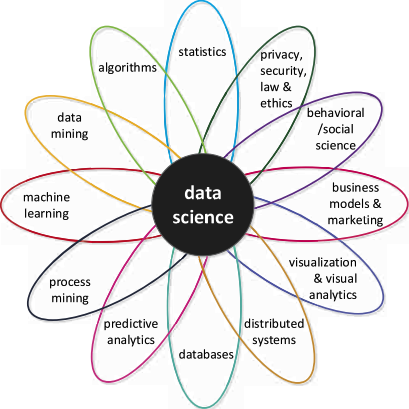
\includegraphics[width=0.5\textwidth]{graphics/ds_disciplines.png}
    \caption{Disziplinen der Data Science}
    \label{fig:data science disciplines}
\end{figure}

Anwendung der Data Science und deren Subdisziplinen findet sich in der Bearbeitung von datengetriebenen Problemstellungen der vier Kategorien: Berichterstattungen, Diagnosen, Vorhersagen und Empfehlungen. \footcite[Vgl.][S. 10]{vanderAalst.2016}
Als Arbeitsablauf dieser Bearbeitung wird in der Literatur häufig ein Prozessmodel mit drei Phasen und bis zu zehn Schritten beschrieben, welcher die Phasen der Datenvorbereitung, der Modellentwicklung und dessen Bereitstellung involviert. \footcite[Vgl.][S. 1]{Zhang.2020b}
Dabei ist es sinnvoll, je nach Anwendung und Problemstellung verschiedene Phasen zu fokussieren.
Beispielsweise sind zur Berichterstattung die Datenvorbereitung und Bereitstellung der Erkenntnisse zu fokussieren, da häufig kein explizites Modell zu entwickeln ist.
Hingegen werden bei der Erstellung von Vorhersagen und Empfehlungen akkurate Modelle benötigt, um die Richtigkeit der Vorhersagen und Empfehlungen zu garantieren.
Konkrete Aufgaben in der Data Science Rolle umfassen das Bereinigen und Vereinen von Datensätzen, die Visualisierung von Daten oder die Entwicklung umfangreicher Softwaretools zur Verarbeitung von Daten. \footcite[Vgl.][S. 13]{Patil.2011}
Das Produkt der Phasen und konkreten Aufgaben kann dabei als analytisches System in einer Organisation betrachtet werden, welches sich aus der Infrastruktur, den Modellen und insgesamt deren Betrieb zusammensetzt. \footcite[Vgl.][S. 22]{Grossman.2014}
Neben dem bekanntesten Anwendungsbereich der Kundenintelligenz kommen derartige analytische Systeme auch im Bereich von Lieferketten- und Qualitätsmanagement sowie Risikoanalyse und Betrugsdetektion zum Einsatz. \footcite[Vgl.][S. 221ff.]{Elgendy.2014}
% Tools
% Zur Umsetzung dieser Aufgaben der unterschiedlichen Phasen werden existieren eine Vielzahl von Werkzeugen und Technologien.

\chapter{Data Science in datengesteuerten Organisationen}

Inhalt dieses Kapitels ist die Darstellung des aktuellen Stands der Forschung zur Eingliederung von Data Science Teams in datengesteuerten Organisationen.
Damit wird verfolgt, ein aktuelles Zielbild annäherungsweise zu konkretisieren, um in weiteren Kapiteln auf die Möglichkeiten zur Integration einzugehen.

Eine Herausforderung entsteht bereits dabei, dass datengesteuerte Organisationen, in der Fachsprache als \textit{data driven Organizations} bezeichnet, einer Vielfalt an Definitionen unterliegen. \footcite[Vgl.][S. 4]{Dalpiaz.2020}
\Citeauthor*{Fabijan.2017} definierte z. B., dass datengesteuerte Organisationen Daten akquirieren, verarbeiten und Datenvorteile in einer zeitlich angebrachten Art und Weise nutzen, um Effizienzgewinne zu erzeugen, neuartige Produkte zu entwickeln und sich durch die Wettbewerbslandschaft zu navigieren. % \footcite[Vgl.][S. ]{Patil.2011}
% insert second definition
Ein gemeinsames Verständnis der Definitionen besteht in dem Prozess des Sammelns von Daten, der Gewinnung von Erkenntnissen durch Analysen und dem Treffen von Entscheidungen basierend auf den erzielten Analyseergebnissen. \footcite[Vgl.][S. 4]{Dalpiaz.2020}
Einer der wichtigsten Aspekte einer datengesteuerten Organisation ist die Manifestation einer datengesteuerten Kultur. \footcite[Vgl.][S. 15]{Dalpiaz.2020}
Dessen Antrieb ist es, Daten nicht nur den Analytic-Abteilungen oder dem leitenden Management vorbehalten sind, sondern so weit wie rechtlich möglich, jedem Organisationsmitglied zur Verfügung gestellt werden sollte. \footcite[Vgl.][S. 6]{Patil.2011}
Dieser Umgang würde es ermöglichen, alle Arten der Analyse (deskriptiv, prädiktiv, präskriptiv) auf allen Ebenen der Organisation (operativ, taktisch, strategisch) einzusetzen. \footcite[Vgl.][S. 4]{Dalpiaz.2020}
In der bisherigen Praxis wird von diesen Möglichkeiten jedoch nur ein Teil angewendet. \footcite[Vgl.][S. 4]{Dalpiaz.2020}
Weitere Aspekte einer datengesteuerten Organisation konnten durch die Forschung von \Citeauthor*{MariusHupperz.2021} identifiziert werden.
Für den untersuchten Aspekt der Data Science ist erkannt worden, dass der Wertbeitrag durch Transparenz, zielgerichtetem Marketing oder automatisierten informierten Entscheidungen zu Wettbewerbsvorteilen führen kann, jedoch keinen unmittelbaren Einfluss auf die Vermögenswerte ausübt. \footcite[Vgl.][S. 5]{MariusHupperz.2021}
Zusätzlich kann Einrichtung einer Digitalisierungsabteilung zwar die Transformation zum datengesteuerten Unternehmen unterstützen, jedoch durch das alleinige Einrichten von Data Science Abteilungen keine Geschäftserkenntnisse aus Daten zu erzeugen. \footcite[Vgl.][S. 5]{MariusHupperz.2021}
Alle weiteren Aspekte aus der strukturierten Literaturanalyse von datengesteuerten Organisationen sind in folgender Abbildung 3.1 dargestellt:\footcite[Vgl.][S. 4]{MariusHupperz.2021}

\begin{figure}[htb]
    \centering
    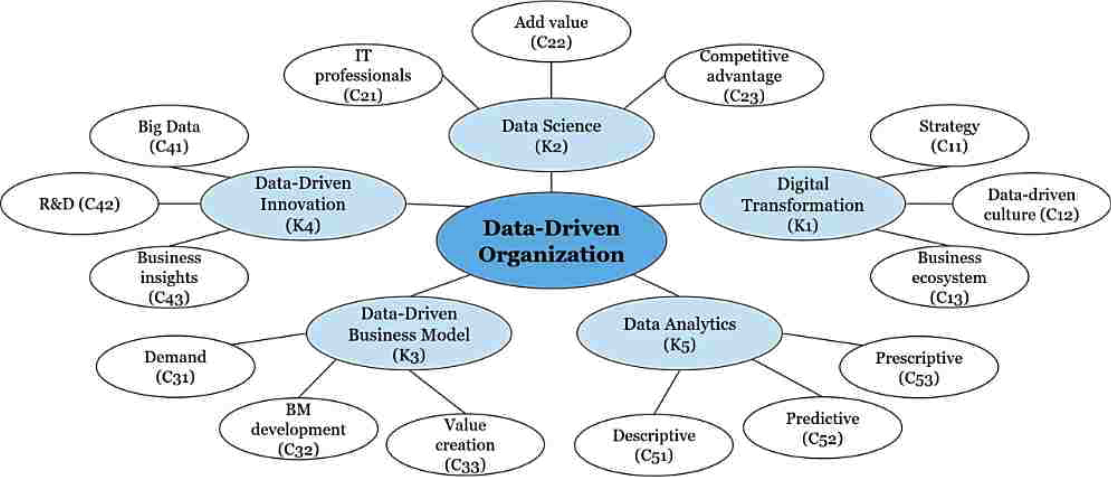
\includegraphics[width=0.95\textwidth]{graphics/ddo aspects.png}
    \caption{In der Literatur beschriebene Aspekte von datengesteuerten Organisationen}
    \label{fig:DDOs aspects}
\end{figure}

Zur praktischen Umsetzung von datengesteuerten Unternehmen führten \Citeauthor*{Zhang.2020b} eine Online Befragung mit insgesamt 183 Teilnehmenden aus der Data Science durch.
Da alle Beteiligten der Umfrage aus dem IT-Konzern IBM stammen, ist die Umfrage zwar nicht statistisch repräsentativ für alle Organisationen zeigt jedoch ein signifikantes Bild über den Aufbau und die Zusammenarbeit von Data Science Abteilungen.
Mit der Umfrage sind Erkenntnisse erzielt worden, welche die fachliche, personelle und Rollen bezogene Zusammensetzung und Zusammenarbeit von Data Science Abteilungen betreffen.
Ein Ergebnis der Umfrage ist es, dass Data science Abteilungen häufig mit einer Teamgröße von bis zu sechs Personen arbeiten, wobei jede Person bis zu 5 Jahre Erfahrung mit Data Science Projekten aufweisen kann. \footcite[Vgl.][S. 7]{Zhang.2020b}
Dabei führen die Teammitglieder meistens mehr als eine Rolle aus, was aus der nachträglichen Abbildung 3.2 (a) hervorgeht: \footcite[Vgl.][S. 7]{Zhang.2020b}

\begin{figure}[h]
    \centering
    \begin{subfigure}[b]{0.45\textwidth}
      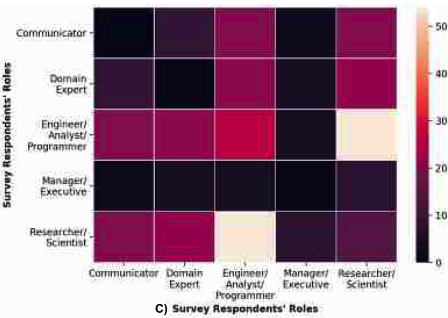
\includegraphics[width=\textwidth]{graphics/ds team roles.png}
      \caption{Häufigkeit der gemeinsam auftretenden Rollen in Data Science Teams}
      \label{fig:heatmap roles}
    \end{subfigure}
    \hfill
    \begin{subfigure}[b]{0.45\textwidth}
      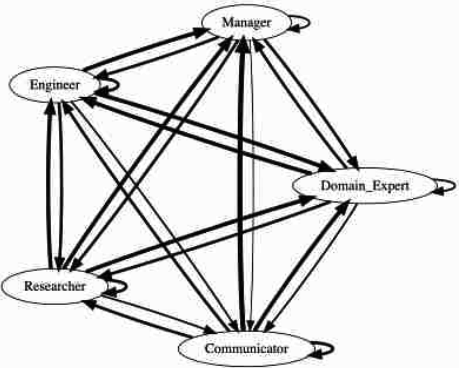
\includegraphics[width=\textwidth]{graphics/ds team network .png}
      \caption{Beziehungsgraph der Zusammenarbeit einzelner Rollen in Data Science Teams}
      \label{fig:network graph}
    \end{subfigure}
    \caption{Rollen und deren Zusammenarbeit in Data Science Teams}
    \label{fig:both_figures}
\end{figure}

Aus der Heatmap wird deutlich, dass die Kombination der Rollen \textit{Researcher - Engineer} am Häufigsten auftritt.
Dies resultiert vermutlich daraus, dass sich in der recht jungen Disziplin der Data Science noch wenig Standards etablierten, wodurch viele Konzepte in Projekten erstmalig zu entwickeln sind.
Durch die Diagnose der Abbildung, in welcher die Häufigkeit von einzeln vorkommenden Rollenbesetzungen abgetragen ist, wird ersichtlich, dass die \textit{Engineer} Rolle häufiger als alle anderen von einer Person ausgefüllt wird.
Daraus lässt sich vermuten, dass der hohe Entwicklungsaufwand in Data Science Projekten die Fokussierung von Personal zur \textit{Engineer} Rolle rechtfertigt.
Als Person in der Rolle des Managers werden, mit Ausnahme der \textit{Researcher} Rolle, noch seltener weitere Rollen ausgeübt, jedoch auch selten lediglich Aufgaben der eigenen Rolle übernommen.
Begründbar erscheint dies durch die Annahme, dass das Management häufig Aufgaben außerhalb des direkten Geschehens im Data Science Projekt umfasst.
Die Ausnahme der \textit{Researcher} Rolle würde sich logisch durch den gemeinsamen hohen Bedarf an Arbeitserfahrung im Themenfeld begründen lassen.

Abbildung 3.2 (b) zeigt den Umfang der Zusammenarbeit zwischen den verschiedenen Rollen auf.
Auffälligkeiten in der Grafik umfassen die Rolle des \textit{Communicators} und des \textit{Domain Experts}.
Die Rolle des \textit{Communicators} wird dabei vermutlich häufig sehr extrovertiert gestaltet, da hier besonders viel ausgehende Zusammenarbeit zu den anderen Rollen erkennbar ist, im Vergleich zu dessen Abhängigkeit.
Etwas gegensätzlich dazu zeigt sich die Rolle des \textit{Domain Experts}, welcher eine starke Abhängigkeit anderer Rollen abbildet, obwohl dabei wesentlich weniger technische Expertise zu erwarten ist.

% anschließend die Collaboration Points anbringen
In datengesteuerten Organisationen gilt es für eine Data Science Abteilung nicht nur innerhalb von sich selbst zusammenzuarbeiten, sondern auch z. B. Komponenten für maschinelles Lernen mit anderen Stakeholdern nutzbar zu gestalten.
Dazu sind vielerlei Punkte in der Abstimmung beider Teams notwendig, wie bspw. Anforderungserhebung, Trainingsdaten und Modellintegration, dessen bewährte Praktiken nachfolgend detaillierter betrachtet werden.
% requirement definition
In der anfänglichen Phase der Anforderungserhebung ist es zum einen wichtig Data Scientists früh in die Definition der Produktanforderungen einzubinden, jedoch zum anderen die Anforderungen an das zu entwickelnde Modell nicht losgelöst des Produkts zu betrachten. \footcite[Vgl.][S. 418]{Nahar.2022}
Die Zusammenarbeit kann zusätzlich unterstützt werden, indem zum einen technische Schulungen für Stakeholder wie Kunden, Produktteams und Endnutzer eingerichtet werden und zum anderen das gemeinsame Verständnis der Anforderungen bestmöglich dokumentiert wird. \footcite[Vgl.][S. 418]{Nahar.2022}
% training data 
Während der Abstimmung der Trainingsdaten mit anderen Abteilungen profitiert der Projektfortschritt, wenn Data Science Teams die Freiheit besitzen, Erwartungen bezüglich z. B. Datenqualität an Lieferanten zu stellen. \footcite[Vgl.][S. 420]{Nahar.2022}
Sollte aufgrund der Projekt- oder Organisationsgröße eine direkte Zusammenarbeit mit dem Datenlieferanten nicht umsetzbar sein, bleibt es notwendig, entsprechende Erwartungen in formalen Verträgen festzuhalten. \footcite[Vgl.][S. 420]{Nahar.2022}
% product model integration
Nach den bisherigen Abstimmung und der Entwicklung des Produkts bleibt der kontinuierliche Prozess des Betriebs.
Die Qualitätssicherung spielt in dieser Phase eine signifikante Rolle und sollte geplant und mit Schulungen zu Themen wie \textit{DevOps} und \textit{MLOps} unterstützt werden. \footcite[Vgl.][S. 423]{Nahar.2022}

% Folgend werden Herausforderungen und Vorgehen behandelt, wie eine Transformation zur datengesteuerten Organisation gelingt, sodass Geschäftsmehrwert aus solcher Arbeit entsteht.

\chapter[Herausforderungen]{Herausforderungen}

Anschließend an die Beschreibung einer datengesteuerten Organisation, dessen Aufbau, Prozesse und Rollen, werden in diesem Kapitel die Herausforderungen zur Transformation in eine datengesteuerte Organisation thematisiert.

Bereits durch das äußere, sich schnell wechselnde kompetitive Umfeld einer Organisation, verkompliziert sich der Prozess datengesteuert z. B. Strategieentscheidungen in Organisation zu treffen. \footcite[Vgl.][S. 2]{Pratt.2023} 
Zusätzlich zu der Geschwindigkeit der Geschäftsumgebung, konnte durch eine Gartner Umfrage festgestellt werden, dass 65 \% der Teilnehmenden im Zeitraum der letzten zwei Jahre (2021-2023) einen Zuwachs der Komplexität von Entscheidungen verzeichneten. \footcite[Vgl.][S. 65]{Pratt.2023}
Damit ist das datengestützte Ableiten von Strategieentscheidungen ein besonders herausforderndes Feld aufgrund der hoch diversen Daten und der Vielzahl von Einflussvariablen. \footcite[Vgl.][S. 3]{Pratt.2023}
Diese äußeren Einflüsse wirken sich ebenfalls erschwerend auf interne managementbezogene und kulturelle Herausforderungen des Transformationsprozesses aus. \footcite[Vgl.][S. 15]{Dalpiaz.2020}
Bestätigt wird dies durch die Forschungsergebnisse von \Citeauthor*{Dalpiaz.2020}, welche 15 Interviews aus neun verschiedenen Softwareunternehmen auswerteten.
Aus den Interviews konnten die folgenden in Abbildung 4.1 dargelegte Herausforderungen in der Transformation zu einer datengesteuerten Organisation identifiziert werden. \footcite[][S. 9]{Dalpiaz.2020}

\begin{figure}[htb]
    \centering
    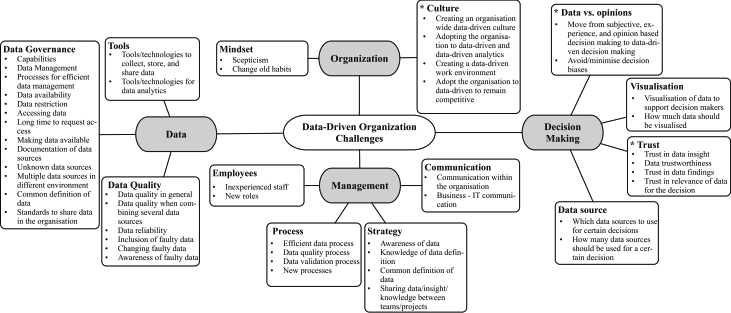
\includegraphics[width=0.95\textwidth]{graphics/DDO challenges.png}
    \caption{Herausforderungen einer datengesteuerten Organisation}
    \label{fig:DDOs challenges}
\end{figure}

Innerhalb der Grafik sind mittels \textbf{*} die drei wichtigsten Herausforderungen gekennzeichnet, welche alle 15 Teilnehmenden benannten: faktenbasierte Entscheidungen, Vertrauen und Kultur.
Faktenbasierte Entscheidungen beschreiben die Absicht, subjektive, erfahrungsgestützte und meinungsbasierte Entscheidungen durch die Nutzung von Daten durchzuführen oder bisherige Prozesse zu unterstützen. \footcite[Vgl.][S. 9]{Dalpiaz.2020}
Ein Einfluss auf die Umsetzung nimmt die zweite Herausforderung des Vertrauens.
Für faktenbasierte Entscheidungen ist ein hohes Maß an Vertrauen gegenüber vielerlei Aspekte der Daten, entlang des Data Science Prozesses, notwendig.
Diese Aspekte umfassen die Aufnahme relevanter Daten, die fehlerfreie Aufnahme der Daten, die fehlerlose Verarbeitung der Daten sowie die korrekte Ableitung von für die Entscheidung relevanten Erkenntnissen. \footcite[Vgl.][S. 10]{Dalpiaz.2020}
Die Aufnahme relevanter Daten wird dadurch herausfordernd, dass in etwa 10 \% der Daten insgesamt 90 \% des strategischen Werts enthalten. \footcite[Vgl.][S. 3]{Pratt.2023}
Neben der Geschäftsleitung ist ein Vertrauen gegenüber Daten und dessen Auswertung auch als gelebte Kultur der Organisation notwendig. \footcite[Vgl.][S. 4]{Dalpiaz.2020}
Eine gelebte datengesteuerte Kultur kann durch eine geringe Akzeptanz neuer Softwaretools und neuer Arbeitsmethoden verhindert werden. \footcite[Vgl.][S. 15]{Dalpiaz.2020}

Eine notwendige Tool gestützte Arbeitsweise ist z. B. die Dokumentation der Zusammenarbeit innerhalb des Teams und mit anderen Abteilungen. \footcite[Vgl.][S. 12]{Zhang.2020b}
Innerhalb dieser Dokumentation können z. B. Lösungen für technische Herausforderungen von der Datenbeschaffung bis zum Modelleinsatz festgehalten werden. \footcite[Vgl.][S. 23]{Grossman.2014}
Im Kontext von großen Datenumgebungen müssen technische Herausforderungen gelöst werden, welche zum einen die Aufnahme aller Daten betreffen. \footcite[Vgl.][S. 217]{Elgendy.2014}
Zum anderen ist die Flexibilität zu gewährleisten, neue Datenquellen einfach anzubinden und Auswertungen schnell durchführen zu können. \footcite[Vgl.][S. 217]{Elgendy.2014}
Durch Hinzunahme von Technologien, wie maschinelles Lernen zur Auswertung von Daten steigen ebenfalls die technischen Herausforderungen.
Maschinelles Lernen bedarf Testsysteme zum Einsatz von Modellen, anpassbare Software zur Überwachung der Modellleistung und Möglichkeiten zur Erläuterung der Modellergebnisse. \footcite[Vgl.][S. 1]{Nahar.2022}

Im gesamten Verlauf der Datenbeschaffung, Modellentwicklung und Ableitung von neuen Optimierungsprozessen sind diverse Teams erforderlich, um vorurteilsbehaftete Datenverarbeitung zu vermeiden. \footcite[Vgl.][S. 18]{Zhang.2020b}
Die Beschaffung von Arbeitskräften für ein solches diverses Team stellt eine weitere Herausforderung dar. 
Hierfür werden Bewerber mit datenbezogener Vergangenheit aus unterschiedlichen Branchen, oder Universitätsabsolventen und ein ausgearbeitetes Einarbeitungsprogramm benötigt. \footcite[Vgl.][S. 13]{Patil.2011}

Diese Herausforderung allein, sowie in Kombination mit den anderen thematisierten Herausforderungen bedarf eines Rahmenprogramms zur Integration von Data Science in verschiedenste Institutionen. \footcite[Vgl.][S. 1]{Saltz.2017}

\chapter[Integrationsprozesse]{Integrationsprozesse}

Nach den behandelten Herausforderungen werden in diesem Kapitel Möglichkeiten und Vorgehensmodelle zur Integration von Data Science in Organisationen thematisiert.
Dazu werden insgesamt drei Modelle der Forschungsliteratur dargelegt.

\section{CSPG Framework}

\Citeauthor*{Grossman.2014} veröffentlichte 2014 das CSPG Framework zur Integration von Analytik, Domänenwissen und IT in Organisationen.
\textit{CSPG} steht repräsentativ als Abkürzung für die Komponenten \textit{Culture, Staffing, Processes} und \textit{Governance}. 
Der Aspekt der Kultur ist durch die Organisationsleitung umzusetzen, indem Verantwortung und Autorität für Datenbestände an eine Funktionsstelle übergeben wird.
Die Aufnahme von Data Science Personal ist im CSPG Framework unausweichlich und durch den Analytik Leiter und die Geschäftsleitung durchzuführen. 
Dabei ist zu entscheiden, ob die analytische Funktion zentral, dezentral oder hybrid organisiert wird.
Im dritten Aspekt des Frameworks sind die analytischen Prozesse in der Organisation aufzubauen.
Ein Teil dieser Prozesse umfasst den Austausch von Daten zwischen Abteilungen und anderen Organisationen.
Weitere Prozesse behandeln die Digitalisierung bestehender Inhalte, Produktanpassung zur Aufnahme von Daten und die Kombination von Datenbeständen.
Die finale Komponente des Frameworks ist der Aufbau, die Verwaltung und die Weiterentwicklung der notwendigen Infrastruktur.
Zur Bewältigung dieser Aufgabe sind die folgenden vier Bedingungen in der Organisation zu erfüllen:

\begin{itemize}
    \item Langfristige Verpflichtung für Data Science und Sicherstellung des daraus entstehenden Geschäftswerts.
    \item Sichere und rechtlich unbedenkliche Umsetzung der Data Science Prozesse.
    \item Herstellen von Haftbarkeit, Transparenz und Rückverfolgbarkeit für Projektfinanzierung, Entwicklung und Ressourcen.
    \item Ressourcenbereitstellung für Daten-, Analyse- und Managementprozesse.
\end{itemize}

\section{Design Parameters}

Durch die Arbeit von \Citeauthor*{JanineAdinaHagen.2020} konnten die Gestaltungsparameter einer datengesteuerten Organisation ermittelt werden.
Diese Parameter können als Richtlinien betrachtet werden, wie die eigene Organisation in verschiedenen Aspekten zu gestalten ist.

\begin{figure}[htb]
    \centering
    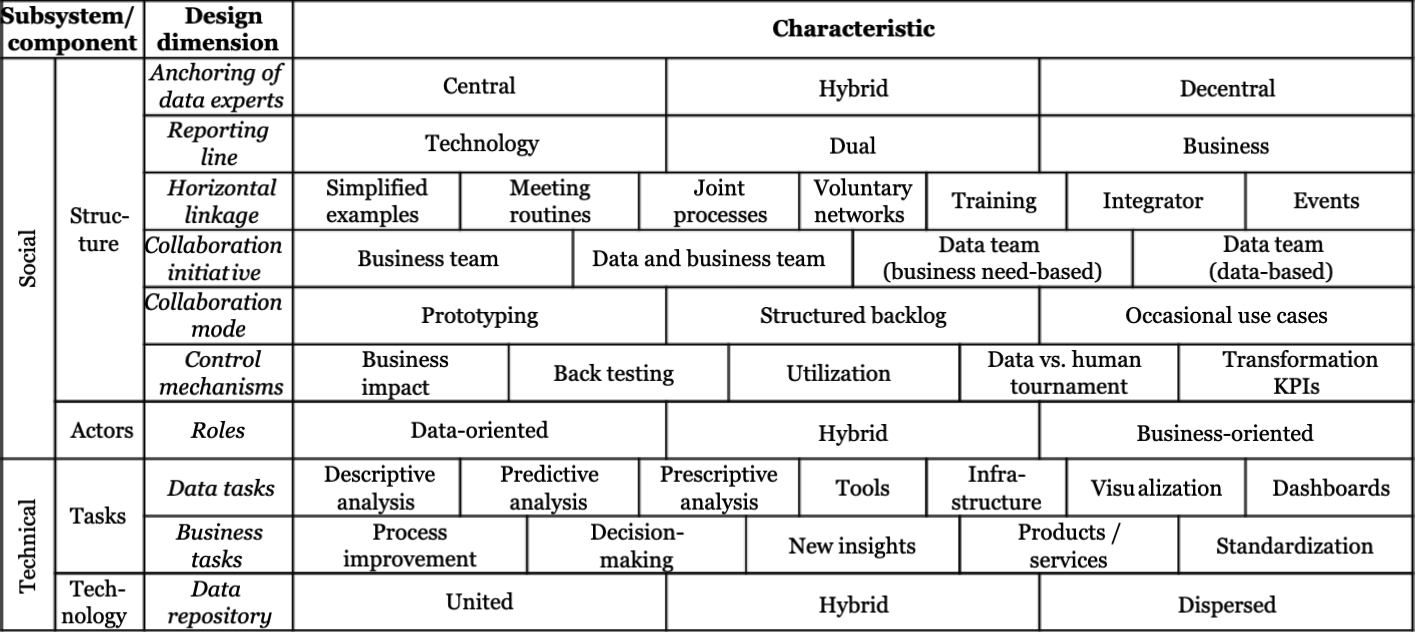
\includegraphics[width=0.75\textwidth]{graphics/DDO_design.png}
    \caption{Gestaltungsparameter einer datengesteuerten Organisation}
    \label{fig:DDOs design}
\end{figure}

Die vorherige Tabelle zeigt die Gestaltungsparameter organisiert nach Komponenten, Dimensionen und konkreter Charakteristika. \footcite[Vgl.][S. 5]{JanineAdinaHagen.2020}
Eine wichtige Komponente betrachtet die soziale Perspektive auf die Struktur und die Akteure der datengesteuerten Organisation.
Die Struktur der Organisation kann durch die Parameter \textit{Expertenorganisation, Berichtslinie, horizontale Verknüpfung, Kooperationsinitiative, Kooperationsmodus} und \textit{Kontrollmechanismus} beeinflusst werden.
Eine mögliche Ausprägung dieser Parameter umfasst z. B. zum einen dezentrale Data Science Experten, eine Berichtslinie zur Fachabteilung sowie regelmäßige Meetings und Events der Data Science Experten.
Zum anderen werden z. B. durch die Datenexperten die Zusammenarbeiten mittels strukturiertem Backlog initiiert und anhand des Geschäftsmehrwerts evaluiert.
In dieser Struktur könnten dann die Rollen z. B. hybrid, also datenorientiert sowie geschäftsorientiert gestaltet werden.
Wird die technische Perspektive betrachtet, werden dessen Komponenten der Aufgaben und Technologien durch die Parameter \textit{Datenaufgaben, Geschäftsaufgaben} und \textit{Datenrepository} bestimmt.
Beispielhaft könnte eine Organisation durch ihre Struktur und Akteure beschreibende, prädiktive und vorhersagende Analysen erstellen, um Prozesse zu verbessern und Entscheidungen zu unterstützen.
Speicherorte für Daten und Software können z. B. hybrid für jedes Datenteam einer Fachabteilung und für den gemeinsamen Austausch mehrerer Datenteams eingerichtet werden.

\section{Experiment Evolution Model}

Ein weiteres Vorgehensmodell durch \Citeauthor*[][]{Fabijan.2017} beschreibt den Transformationsprozess von Ad hoc Analysen zu skalierten kontrollierten Experimenten in Organisationen. \footcite[Vgl.][S. 5]{Fabijan.2017}
Das Experiment Evolution Modell verdeutlicht die Evolutionsphasen datengesteuerter Entwicklung in Unternehmen und Abteilungen.
Zur Anwendung des Modells sind Voraussetzungen zu erfüllen, welche folgend thematisiert werden.

Eine Anwendung setzt insoweit Fähigkeiten der Data Science voraus, sodass Produktstatistiken evaluiert werden können.
Die Fähigkeiten umfassen das Verständnis von Hypothesentests, Randomisierung, Stichprobengrößen und die Berechnung von Konfidenzintervallen. %\footcite[Vgl.][S. 6]{Fabijan.2017}
% Falls derartige Fähigkeiten nicht vorliegen, können Onlineressourcen die Weiterentwicklung der Mitarbeiter unterstützen.
Die Kombination dieser Fähigkeiten mit Domänenwissen ermöglicht die Generierung und Evaluation erster Produkthypothesen.
Als zweite Anforderung wird die Verfügbarkeit eines Zugangs zu Daten der Produktverwendung vorausgesetzt.
% Je nach Domäne können dabei komplizierte Fragestellungen hinsichtlich rechtlicher sowie technischer Herausforderungen aufkommen.

Die im Modell abgebildete Evolution erfolgt in den drei Dimensionen Technisch, Organisatorisch und Geschäftlich. 
Jede Dimension folgt den vier Phasen \textit{Krabbeln, Gehen, Rennen} und \textit{Fliegen}.
Zu Beginn der ersten Phase finden in der technischen Dimensionen der Aufbau von Logging-Systemen und erste manuelle produktspezifische Analysen von Data Science Teams statt.
Die Geschäftsdimension beinhaltet die Definition von unternehmensweiten Evaluationskriterien in Verbindung mit den langfristigen Geschäftszielen.
Während der Phase des \textit{Gehens} werden in der technischen Dimension Metriken entwickelt, anhand dessen Eventdaten aggregiert betrachtet werden können.
Diese Phase erzeugt den Bedarf einer übergreifenden Analyseplattform durch das Wachstum an Experimentarten und Anwendungen. 
In der Organisation bauen während dieser Phase Data Science Experten zunehmend Wissen zu einzelnen Produkten auf.
Ebenfalls werden Daten und Vorgehensweisen weitreichend geteilt.
Die Geschäftsdimension entwickelt sich durch Validierung bestehender und Entwicklung neuer Evaluationskriterien z. B. hinsichtlich der Datenqualität.
Zur Phase des \textit{Rennens} werden in der technischen Dimension Analyseplattformen skaliert und Experimente für mehrere Produktteams ausgeführt, um einen Fokus auf nahverwandte Metriken der Geschäftsziele zu setzen.
Organisatorisch übernehmen Produktteams volle Verantwortung und für ihre Ergebnisse, werden aber noch fachlich von Data Science Experten begleitet.
In der Geschäftsdimension werden bisherige Qualitäts- und Leistungskriterien verfeinert und kombiniert, um Ergebnisse zu Standardisieren und wenige klare Ziele zu fokussieren.
Die letzte Phase des \textit{Fliegens} fokussiert in der technischen Dimension die Standardisierung der Metrikentwicklung, Erweiterung der Plattformautomatisierung und Aufnahme von Daten zu jeder Produktänderung.
Die Evolution der Organisation umfasst zu diesem Zeitpunkt die autonome Durchführung von Analysen durch Produktteams und Entwicklung von Plattformen durch zentrale Data Science Teams.
In der Geschäftsdimension sind zu dieser Phase lediglich periodisch Änderungen an definierten Evaluationskriterien und deren Entwicklungsprozessen vorzunehmen.

Das Modell lässt sich zusammenfassend wie folgt in Abbildung 5.2 darstellen. \footcite[Vgl.][S. 6]{Fabijan.2017}
\begin{figure}[htb]
    \centering
    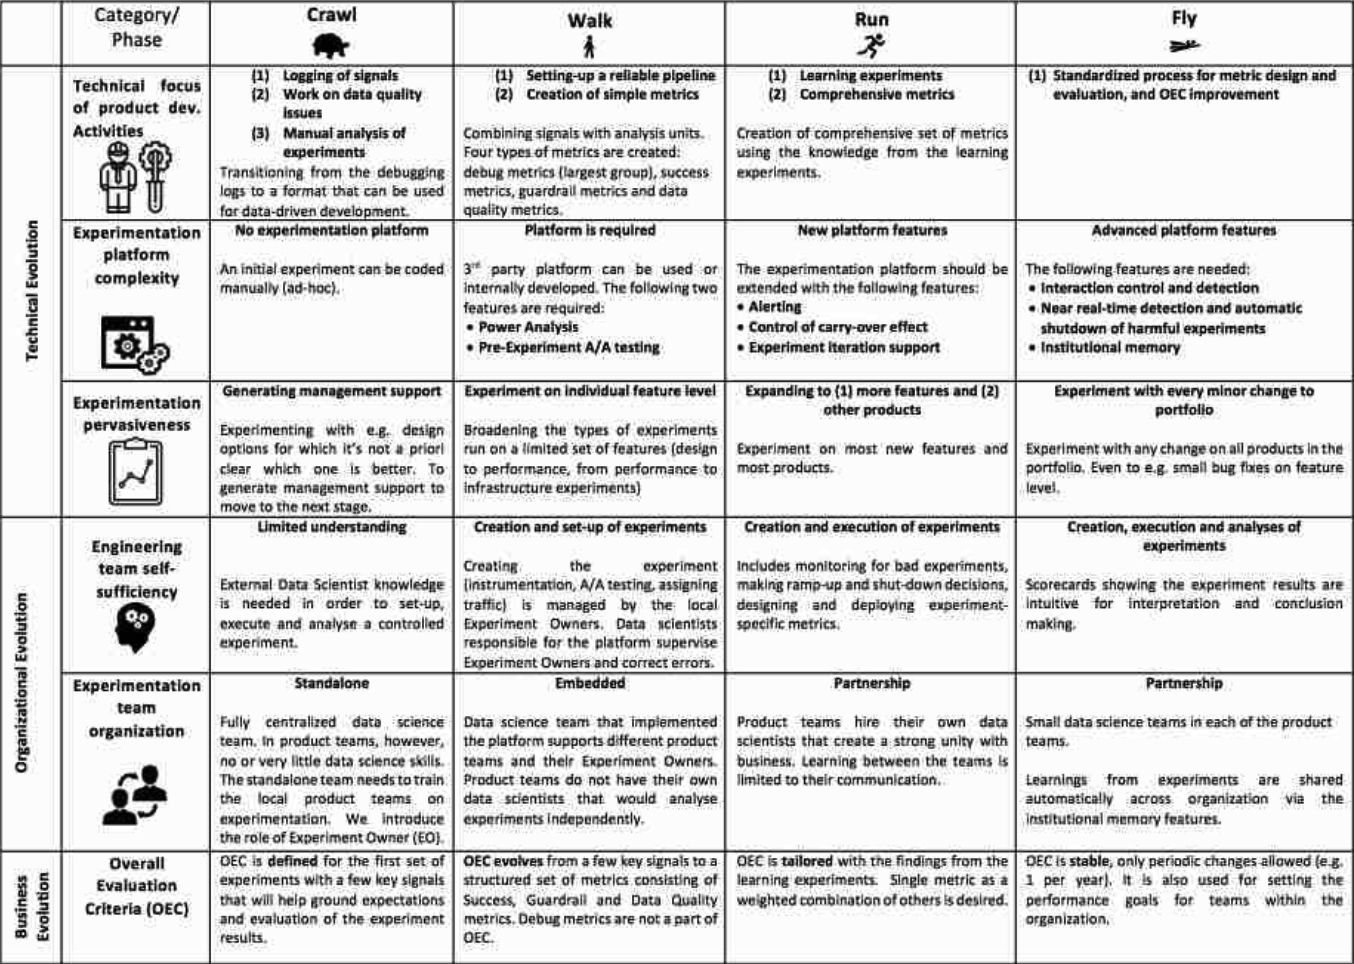
\includegraphics[width=0.67\textwidth]{graphics/EEM model.png}
    \caption{Gestaltungsparameter einer datengesteuerten Organisation}
    \label{fig:EEM model}
\end{figure}
\chapter[Fazit]{Fazit}


\begin{itemize}
    \item Lernleistung lediglich durch Noten bemessen
    \item alter Datensatz
    \item Komplexität ist ok, da durch das digitale format Visualisierungen in den angezeigten Daten gefiltert werden können. (zoom, kategorie auswahl)
\end{itemize}

%Literaturverzeichnis einfügen
\renewcommand*{\UrlFont}{\rmfamily}
\printbibliography
\section*{Eidesstattliche Erklärung}

Hiermit erkläre ich, dass ich die vorliegende Arbeit eigenständig und ohne fremde Hilfe angefertigt habe. Textpassagen, die wörtlich oder dem Sinn nach auf Publikationen oder Vorträgen anderer Autoren beruhen, sind als solche kenntlich gemacht.

Die Arbeit wurde bisher keiner anderen Prüfungsbehörde vorgelegt und auch noch nicht veröffentlicht. \newline

Köln, den \today

\vspace{15mm}

Leon Henne


\end{document}
